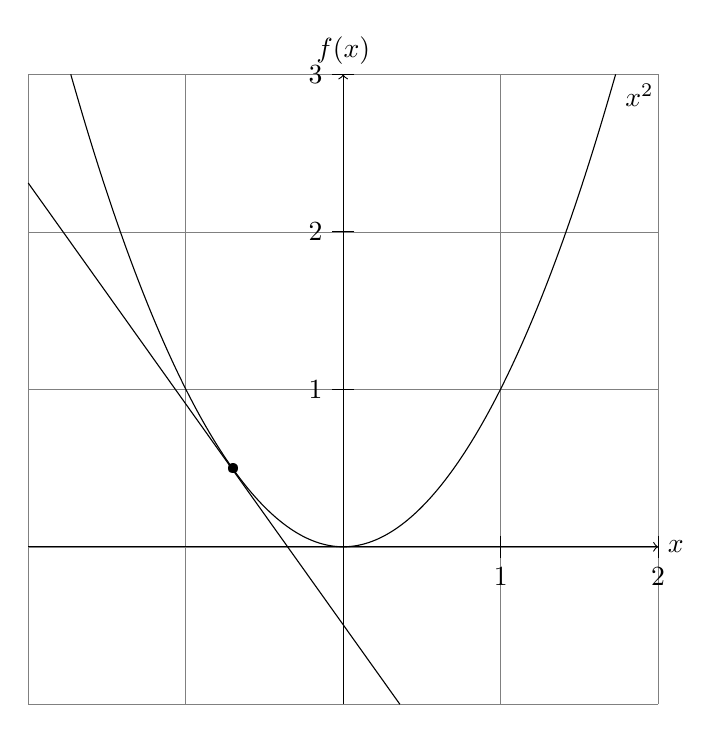
\begin{tikzpicture}[scale=2]
%  \draw[style=help lines] (0,0) grid (3.9,3.9);$
  \draw[style=help lines] (-2,-1) grid (2,3);

  \draw[->] (-2,0) -- (2,0) node[right] {$x$};
  \draw[->] (0,-1) -- (0,3) node[above] {$f(x)$};

  \foreach \x/\xtext in {1/1, 2/2}
    \draw[shift={(\x,0)}] (0pt,2pt) -- (0pt,-2pt) node[below] {$\xtext$};

  \foreach \y/\ytext in {1/1, 2/2, 3/3}
    \draw[shift={(0,\y)}] (2pt,0pt) -- (-2pt,0pt) node[left] {$\ytext$};

  \draw (-1.73,3) parabola bend (0,0) (1.73,3) node[below right] {$x^2$};
  \node at (-0.7, 0.49) {
    \textbullet
  };
  \draw (-2, 2.31) -- (0.36, -1);
\end{tikzpicture}

%% \begin{tikzpicture}[scale=2]
%%   \shade[top color=blue,bottom color=gray!50]
%%       (0,0) parabola (1.5,2.25) |- (0,0);
%%   \draw (1.05cm,2pt) node[above]
%%       {$\displaystyle\int_0^{3/2} \!\!x^2\mathrm{d}x$};

%%   \draw[style=help lines] (0,0) grid (3.9,3.9)
%%        [step=0.25cm]      (1,2) grid +(1,1);

%%   \draw[->] (-0.2,0) -- (4,0) node[right] {$x$};
%%   \draw[->] (0,-0.2) -- (0,4) node[above] {$f(x)$};

%%   \foreach \x/\xtext in {1/1, 1.5/1\frac{1}{2}, 2/2, 3/3}
%%     \draw[shift={(\x,0)}] (0pt,2pt) -- (0pt,-2pt) node[below] {$\xtext$};

%%   \foreach \y/\ytext in {1/1, 2/2, 2.25/2\frac{1}{4}, 3/3}
%%     \draw[shift={(0,\y)}] (2pt,0pt) -- (-2pt,0pt) node[left] {$\ytext$};

%%   \draw (-.5,.25) parabola bend (0,0) (2,4) node[below right] {$x^2$};
%% \end{tikzpicture}
